In our era technology has a fundamental role in almost every field. From the simple communications activities to those related to medical researches, technology is something we cannot do without. It is also a great opportunity in educational field, where it is demonstrated that the so called "stealth learning" (i.e. the help of technologies in educational scope) \cite{Sharp} is a solution to create a greater emotional involvement and that has as a consequence the ability to increase learner's learning opportunities. In our specific case, stealth learning is suitable for the treatment of patients affected by NDD to develop their cognitive, emotional and intellectual skills. Games are already widely used in therapeutic scope, due to the natural attraction people feel about this kind of activities. \\
\\
More recently, some experiences have demonstrated that the use of games in educational scope is something very successful \cite{Mazzone}, due to different aspects:
\begin{itemize}
\item People with NDD are usually really attracted by technological devices and technological gaming experience, and this could be exploited to teach important lessons about various kind of things related to everyday life such as autonomy (eg in food education area).
\item Virtual reality can be seen as a good candidate in the treatment of this kind of people, because it leads to a more focused activity in a simplified real-life context in which patients can improve their skills and then apply them to real life situations.
\end{itemize}


\section{Modern technologies for NDD people}
All the new existing technologies are now helping therapists and families to deal with neurological disabilities. In fact, in addition to virtual reality, smart objects, multisensor environments or smart spaces and conversational agents are used.\\
Smart objects are devices that can interact not only with the user but also with other similar devices and with the surrounding environment. Physical world can be described in terms of three properties \cite{Smart}: awareness (is a smart object to be able to understand events and human activities occurring in the physical world), representation (refers to a smart object's application and programming model) and interaction (denotes the object's ability to converse with the user in terms of input, output, control, and feedback).\\
Examples are Dolphin Sam \cite{Dolphin} and  Huggable \cite{Huggable}. \\
Smart spaces or multisensor environments are rooms in which children can play or interact in a controlled way because they are equipped with techonological items like cameras, smart objects, leds and projectors.
\\
Examples are Magic K room e M4All \cite{M4all}. \\
Conversational agents are devices that can communicate with the user in a manner consistent with what is required: an interaction of the user is answered by the agent who must be with sense.\\
\begin{figure}[H]
\centering
\begin{minipage}[c]{.40\textwidth}

\includegraphics[width=1\textwidth]{immagini/delfino.png}
\end{minipage}%
\hspace{10mm}%
\begin{minipage}[c]{.40\textwidth}
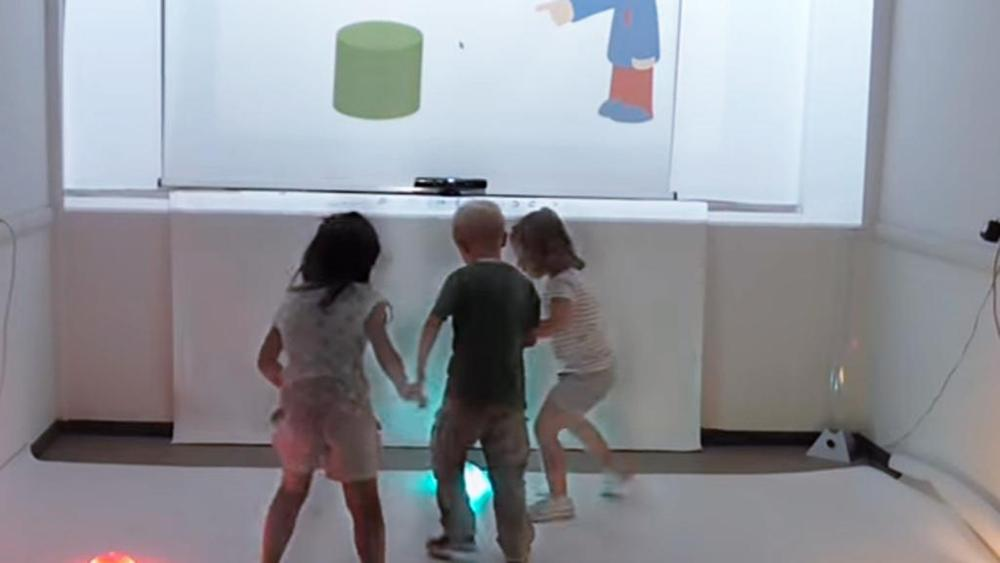
\includegraphics[width=1\textwidth]{immagini/stanzamagica.jpg}
\end{minipage}
\caption{Dolphin Sam and Magic K Room}\label{fig:smartimages}
\end{figure}

\section{Virtual Reality}
The great benefits of using Virtual Reality in an educational and rehabilitation context are now recognized worldwide and tested through various comparative tests between rehabilitation with the use of new technologies and rehabilitation with the use of classical methods \cite{Parsons}, \cite{Reid}, \cite{Wii}. In \cite{Pelagia} a review is carried out on recent literature to support and demonstrate the effectiveness of the use of VR with autistic children and in \cite{Tandra} the effects of a virtual reality game are analyzed to demonstrate the increase in social and emotional activities on a sample of 30 children between 7 and 16 years who suffer from ASD.\\
As previously mentioned, for the development of GEA, an approach that uses Werable Immersive Virtual Reality (WIVR) has been preferred since the possibility of a complete immersion in the environment and the removal of many distractions are the basis of an effective therapy. The user is in a world similar to the real one but safer as there is nothing that can hinder his learning and is reduced to the maximum the "fear" of making mistakes: it is as if the person could "train" the daily life so you can be ready and not catapulted into a world difficult for him. The use of the viewer also allows you to maintain a greater level of concentration because the player can not distract looking elsewhere or perceive the looks and reactions of those around, the only source of disturbance will then be sound. Once this type of games was not accessible to everyone because of the costs of technology and the problems that have been encountered in using it, such as a sense of nausea as sutied by the United States Army in \cite{Eugenia}, but nowadays many steps have been taken and viewers, as well as virtual reality itself, are within everyone's reach.\\
Regarding the technology of Virtual Reality viewers, HMDs, now on the market there is a clear division between two currents: embedded viewers, such as HTC Vive Pro, \cite{Vive}, and modular viewers, such as Google Cardboard, \cite{Cardboard}, and Samsung Gear VR, \cite{Gear}.\\
\textbf{HTC Vive Pro}
\begin{figure}[H]
\centering
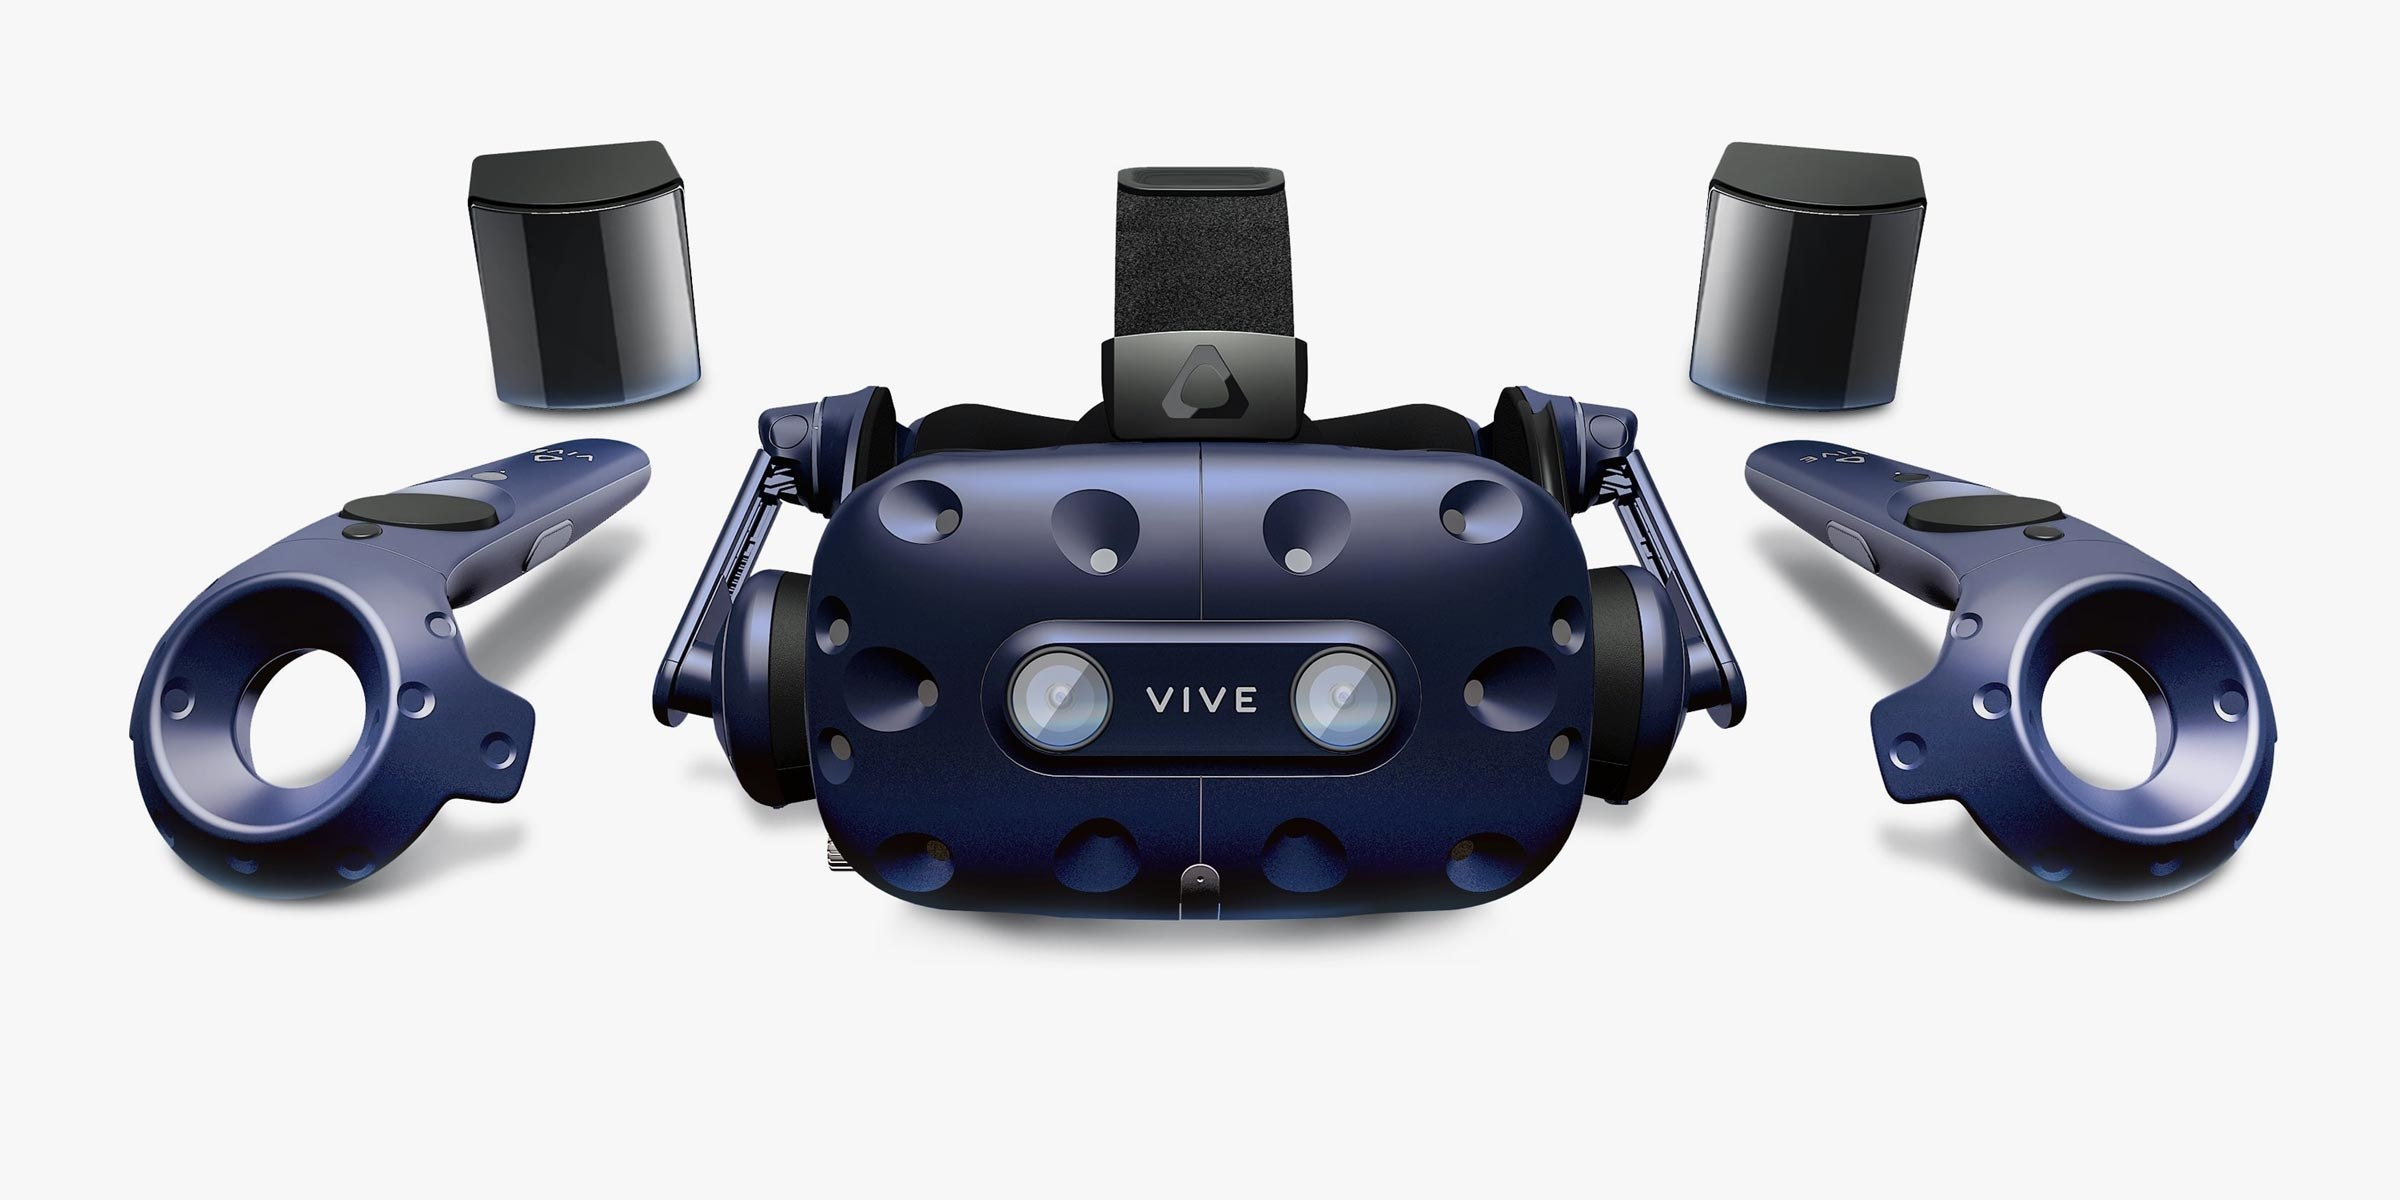
\includegraphics[width=12cm, height=6cm]{immagini/vive.jpg}
\caption{HTC Vive Pro}\label{fig:htcvive}
\end{figure}
HTC Vive Pro is an advanced virtual reality headset developed by HTC and Valve Corporation.The Vive Pro uses two screens, one per eye, each having a display resolution of 1440x1660. The displays are made of AMOLED technology, having a refresh rate of 90 Hz (90 frames per second). The device uses these sensors: SteamVr Tracking, G-Sensor, gyroscope, proximity and IPD sensor. It uses optimized ergonomics and lenses with 110 degrees. But it has a very high cost: 879 euro only the visor and 1399 euro the complete pack (from the official store).\\
\\
\textbf{Google Cardboard}
\begin{figure}[H]
\centering
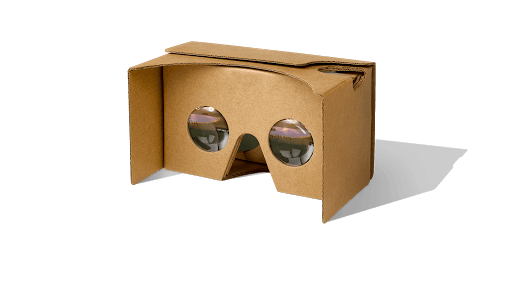
\includegraphics[width=12cm, height=6cm]{immagini/cardboard.png}
\caption{Google Cardboard}\label{fig:cardboard}
\end{figure}
Google Cardboard is composed of two biconvex lenses mounted on a plastic or cardboard frame available in different colors and shapes. The smartphone placed inside this structure shows the visual contents, subdividing them into two-dimensional images with two identical dimensions, and the interaction is obtained through the focused gaze. The user can navigate the virtual world by rotating his head which will consequently rotate the virtual scene projected on the display.\\
\\
\textbf{Samsung Gear VR}
\begin{figure}[H]
\centering
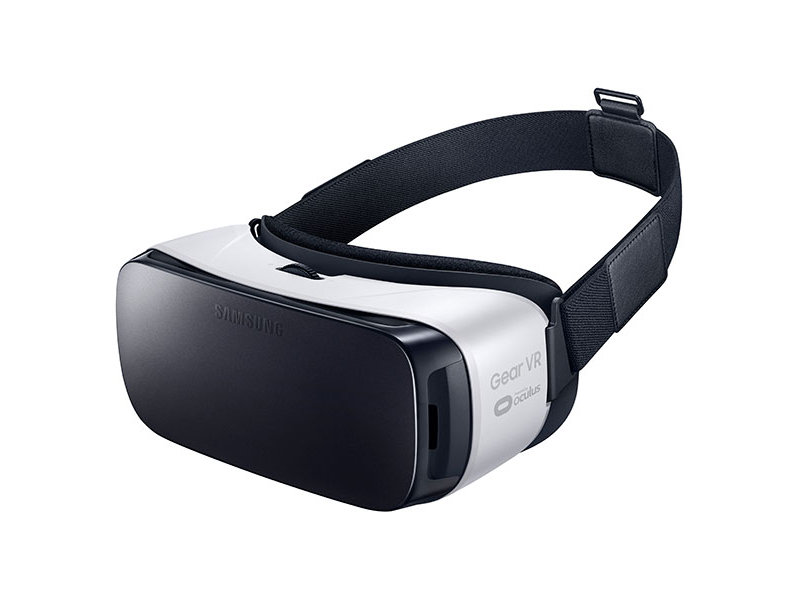
\includegraphics[width=10cm, height=6cm]{immagini/gear.jpg}
\caption{Samsung Gear VR}\label{fig:gearvr}
\end{figure}
Samsung Gear VR is still a modular HMD, produced by Samsung and Oculus VR. It is lightweight and with a good quality of materials,it has accelerometer, gyroscope and proximity Sensor but we can use it only with Samsung smartphones with some specifics. It costs more than Cardboard but it is not so expensive.\\
\\
During the implementation and testing phases of GEA we decided to use the modular visor as it turns out to be the most economical choice on the market and the financial factor is of great importance since the game is designed to be integrated into existing and widely adopted in therapeutic programs.

\section{Touchscreen}
The massive evolution that touchscreen devices have had in recent years, has strongly influenced our way of life. The amount of time a person spend on internet or on electronic devices in general is something that continues to grow every year. From a general point of view this is surely not a good thing because it has a large number of consequences that we have to take care of. \\
This new trend of life surely influences also children, that spend a lot of their time playing games on touchscreen devices, that are more accessible than traditional computers and video games because the motor skills needed to use them are not necessary.\\
\begin{figure}[H]
\centering
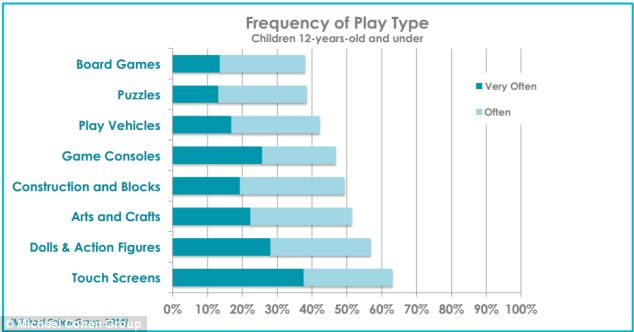
\includegraphics[width=10cm, height=7cm]{immagini/touch.png}
\caption{Time spent by children at playing games}\label{fig:timegames}
\end{figure}
Despite this kind of behaviour is largely criticized and not recommended by doctors and psychologists, the experiment conducted by B. Huber, J. Tarasuik, M.N. Antoniou, C. Garrett, S.J. Bowe and J. Kaufman \cite{Huber} demonstrated that children could learn from touchscreen educational games and apply this knowledge on physical problems. In fact there're a lot of applications thought for this purpose that help children to develop memory, problem-solving and executive functioning skills that could then be applied to real-world problems. The experiment shows substantially that there's no difference in learning for children that use real objects from those who learn only on touchscreen application. In particular, as observed by M.J. Mayo \cite{Mayo}, games could involve children more easily due to the presence of images, animations and sounds. Moreover, they're particularly adept at dosing information delivery. On a touchscreen application it is easy to complicate things and to add visual elements as the difficulty increases, while mantaining the focus on a small area that avoid extraneous distractions, so these educational games seems to be effective in enhancing motivation and increasing children interest in subject matter that leads to more effective learning \cite{Annetta}. 

\section{Projects about food education}
In the specific field of food education, we could find different kinds of game developed for touchscreen devices. In particular one example is the Food pyramid game developed by the Colorado State University \cite{Serrano} as a game to teach children what are the five main food groups and how to apply this knowledge to plan meal and snacks in order to increase their self-efficacy. This game is composed by various challenges regarding the food pyramid, and the researches has concluded that a game composed with a challenge is more effective that one based on a storyline.\\
Important companies are committed every year to the promotion and development of interactive educational games for children in this field both for the school and for the home, it is an example Nestl\'e with the project "Nutrikid", \cite{Nutrikid}, prepared with advice Scientific Committee of the NFI, Nutrition Foundation of Italy. As they read from their website "The Nutrition Foundation of Italy, was constituted legally as a non-profit association in December 1976, with the aim of activating interactions and collaborations with government bodies, universities and industry to contribute the development of scientific research, the exchange of information in the field of nutrition and the promotion of interdisciplinary research in this field.", \cite{NFI}, for this reason we have drawn great inspiration from it during the development of GEA. Other projects in this field are continually promoted by the FEI, Food Education Italy, a foundation of accredited participation at the Ministry of Education, University Research, which lives on voluntary contributions and is involved in helping schools and teachers to develop their role of food educators, \cite{FEI}.\\
Instead, as regards the specific field of food allergies, the state of the art appears to be scarce. It is possible to find, as applications, on the App Store and Play Store, only two games in this regard and both are in English, they are "Wizdy Diner" and "Allergy Reality" developed with touch screen technology and for PC. \cite{Wizdy} and \cite{Allergy}\\
On the website of healthy eating \cite{Myplate} we can find other kind of games related to food education developed for personal computer. One of them "My plate match game" teaches the user to characterize the different kinds of food in a correct diet and how much of every food is needed daily. The objective of this game can be divided into three mini goals:
\begin{enumerate}
\item Fill the plate with different colored shapes related to different kinds of food, this is quite trivial, because it is easy to understand where to put the shapes. At the end, the user could read some explanations about a specific food by putting the cursor on the shapes.
\item This second mini goal is more related to the association food-group. There are various foods and the user must put them in their correct food group.
\item The last goal requires to insert a lot of physical activities in a clock until it reaches a total of one hour. 
\end{enumerate}
\begin{figure}[H]
\centering
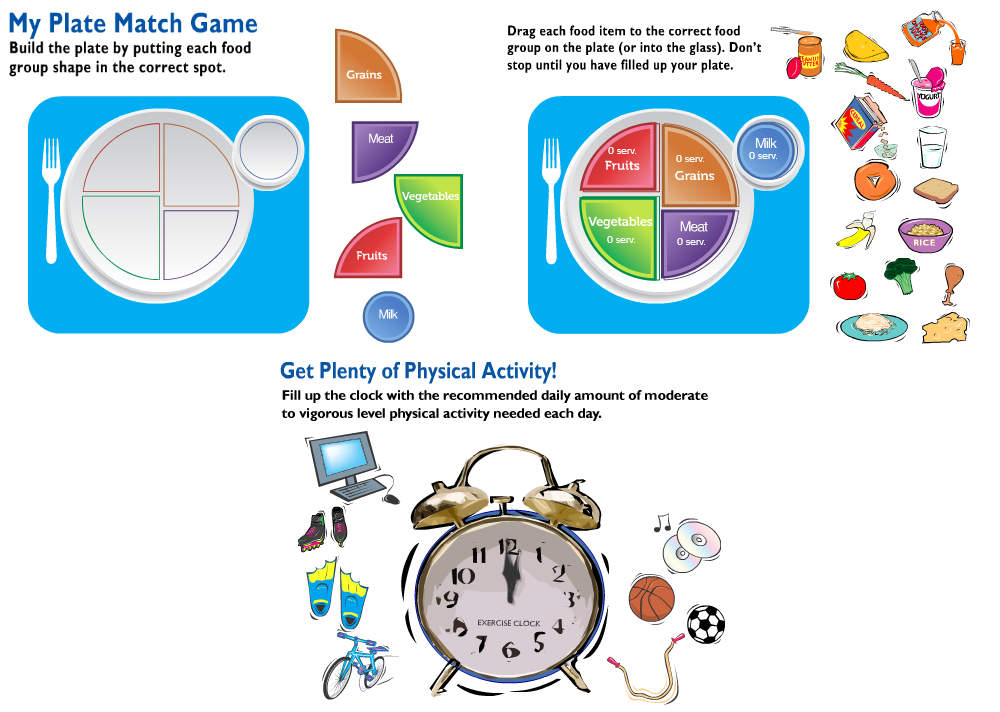
\includegraphics[width=11cm, height=7cm]{immagini/myplate.png}
\caption{My plate match game}\label{fig:myplate}
\end{figure}
This game has not a proper feedback, because it will continue until all the goals are reached correctly (there's not error counting).\\
On the same website there is also another game specifically designed for healthy breakfast, "Power up your breakfast": this game is similar to the previous one, at the beginning the user must answer to some question regarding the importance of breakfast.
The last game we have found is "My very own pizza" that allow the user to build a customized pizza without a true objective (the user could insert all the ingredients he wants).
However, surfing on the internet we have seen that games related to food education in general are quite common, another example we have found is Nourish interactive website \cite{Nourish} that contains a huge amount of games with the food theme.
\section{Projects about food allergies education}
Contrary to what we have seen for food education in general, it is not easy to find previous digital works about the specific field of food allergies. Most of the work, in fact, are paper games based on previous explanations or in-game explanations. The only digital games we have found are on "My kids food allergies" website \cite{Mykids} in the arcade section, however most of the games we have tried does not work, only 3 out of 8 titles can be played.\\
"Supermarket search" is the first game we had faced with: there're three characters, each one has two kinds of food allergies and at the beginning of the game, the user must choose one of them. The chosen character asks the player to help him/her to buy some thing at the supermarket related to the preparation of a specific recipe. The player must choose among two different choices the correct one (the foods alternative could be allergens or things that are not related to the recipe) and the game is completed after five steps. 
\begin{figure}[H]
\centering
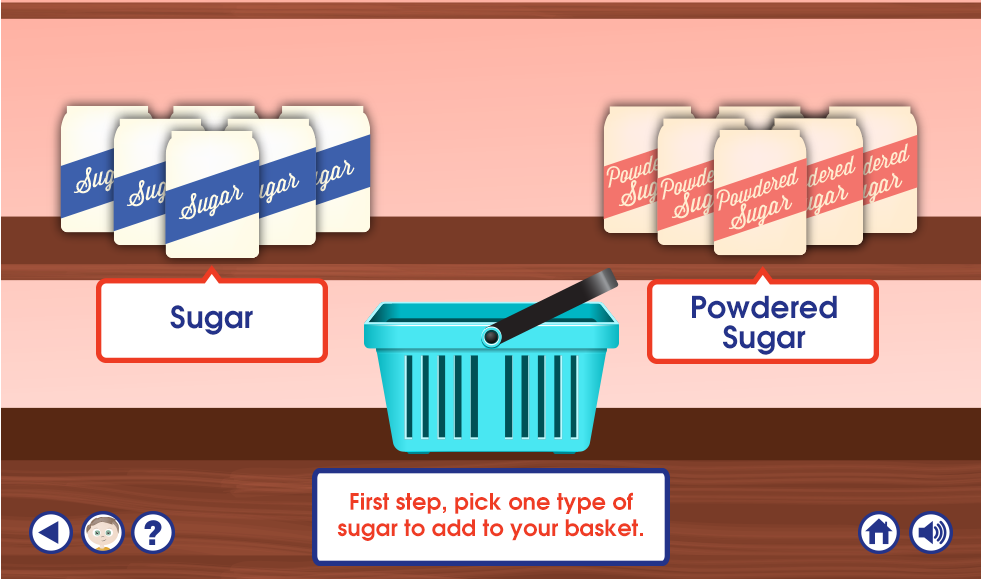
\includegraphics[width=11cm, height=7cm]{immagini/supermarket.png}
\caption{Supermarket search}\label{fig:supermarket}
\end{figure}
The second game we have tried is "food allergy bubble games" in which the user must choose one allergen among seven choices and when the game has started, the user must break the bubbles that contains that specific allergen, by moving a nose that has a needle. It is difficult to choose only the allergens because the bubbles are too much near each other and it's possible to make only three errors.
\begin{figure}[H]
\centering
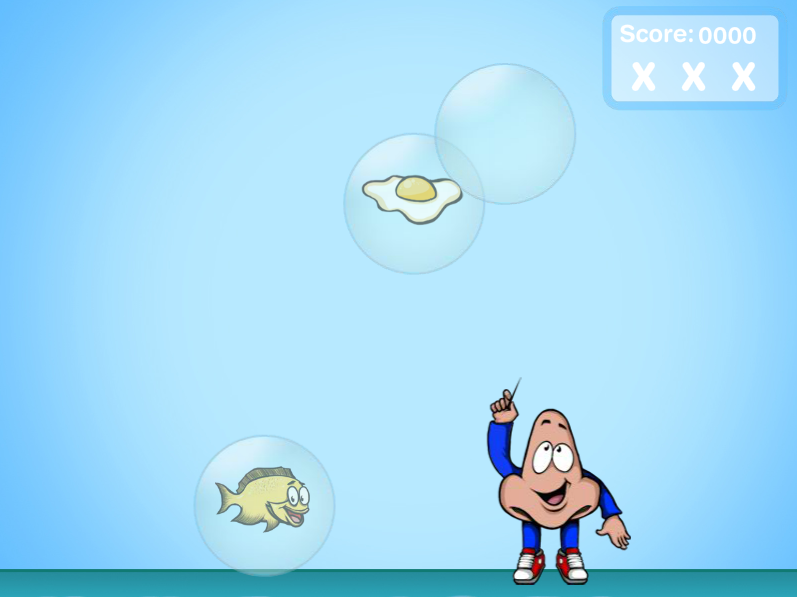
\includegraphics[width=11cm, height=7cm]{immagini/bubble.png}
\caption{Food allergy bubble games}\label{fig:bubble}
\end{figure}
The last working game is based on a memory in which the user must associate the correct image to the word that represents its name, this can be useful to associate a specific allergen to its iconic representation on food boxes.\\
All the other paper games are more related to symptoms of allergies, to their spelling and their consequences.

\section{Participatory Design}
\subsection{What is Participatory Design?}
Participatory design is an approach to design which aim is to involve the final users as active stakeholders and not just as targets or entity of study that tries to guarantee that the final product will meet their needs and that it will be usable. This approach is focused on processes and procedures of design but it is not a proper design style.\\
Recent studies \cite{Val} have proven how designers that works in a co-design fashion creates more innovative products, concepts and idea rather than working on their own and it is clear how the participation of the final users in all the product design phase raise the importance of their opinion that previously were considered only in testing phase. \\
In participatory design, participants are invited to cooperate with designer in different stages of the product design, from the very starting point in which there's idea discussion, where the participants could increase the domain knowledge of the problem (for example if a product will be designed for a certain kind of target, the participation of user belonging to that category will be of great help to understand pro and cons of each idea), during the development in which they evaluate proposed solution, until the final product effective release. Pieters and Maarten \cite{7Princ} describe co-design as a part of the complete co-creation process that refers to the "transparent process of value creation in ongoing, productive collaboration with, and supported by all relevant parties, with end-users playing a central role" and covers all stages of a development process.\\
The approach of participatory design was actually bornt in Scandinavia in the 1970s and at the beginning was called "cooperative design" even if, as the US community which the method was presented to noticed, initially it was something that create a separation between the managers and workers because there weren't sessions that include them both and in which they could discuss and compare their ideas but there were separate meeting without a direct cooperation.\\
Later they understood the importance of previous experience to give the product design something more that allows the reach of major achievement with methods developed through the focus on hands-on experience.
Co-design is often used by trained designers who recognize the difficulty in properly understanding the cultural, societal, or usage scenarios encountered by their user. As Prahalad and Venkat recognized in their book \cite{Cocreate} "The meaning of value and the process of value creation are rapidly shifting from a product and firm-centric view to personalized consumer experiences. Informed, networked, empowered and active consumers are increasingly co-creating value with the firm" and we can see how in the last years the importance of co-design has reached different design fields, in particular the mobile app development.

\subsection{Participatory Design with children}
Participatory design method can involve a wide variety of kinds of people that goes from sportspeople to elder people, so it must consider even children as a valid participant category.\\
Co-design with children is something really important because we have to consider that a wide variety of thing are designed for children: for example games, transports, books and so on. In our specific field it is important to collaborate with children to understand their needs, their wishes and their knowledge to build a suitable educational game.\\
When participatory design implies the presence of a specific category, one must take care of the different requirements that must be satisfied for that kind of people. In particular, when dealing with children, in addition to robustness, reliability, validity, thoroughness and efficiency, one must care that the implied
techniques allow to produce a useful result and - at the same time - that said procedures are appropriate and suitable for children as active participants.\\
One of the most relevant aspects of co-design is that the participants must be really attracted and interested on the design activity and on what the designer are trying to produce because the product will be something that they will use. Children by nature get easily bored and more distracted by an activity, specially if it has going on for a long time and with repeated tasks. It is vital to produce a participatory design session that is immersive for them in order to exploit all their suggestions and impressions. A way to reach this objective is to guarantee that the process is continuously renewed in order to keep the participants' attention and interest level high \cite{PDC1}. With respect to this aspect, many point out that efficient ways of countering the distraction/boredom factor are to make use of a storytelling setting for the sessions, or even to focus the PD process around a game: these two approaches mix together emotional involvement and interactivity, and often improve the way in which children participate in the design process altogether.\\
Another problem that raises from the participatory design with children is the fact that they have limited communication skills, so a session based only on lone verbal and written opinion may result in leaving out some of their suggestions that they don't know how to express. \\
Therefore it is crucial to find other ways to use as communication channels to allow for more complex interactions between participants and design experts that could otherwise be limited by the restrictions on communication itself \cite{PDC2} some researches have underlined the efficacy of more "manual" communication means as drawing and crafting simple objects, the use of tables or of multiple choice sheets. In particular it has been observed how some props are efficient to design a proper communication between the designer and children because they can be seen as a stimulus (maintaining also high level attentions and wander) to design something new. This could lead to exploit multiple children opinions and to raise the level of the design object in analysis.\\
\begin{figure}[H]
\centering
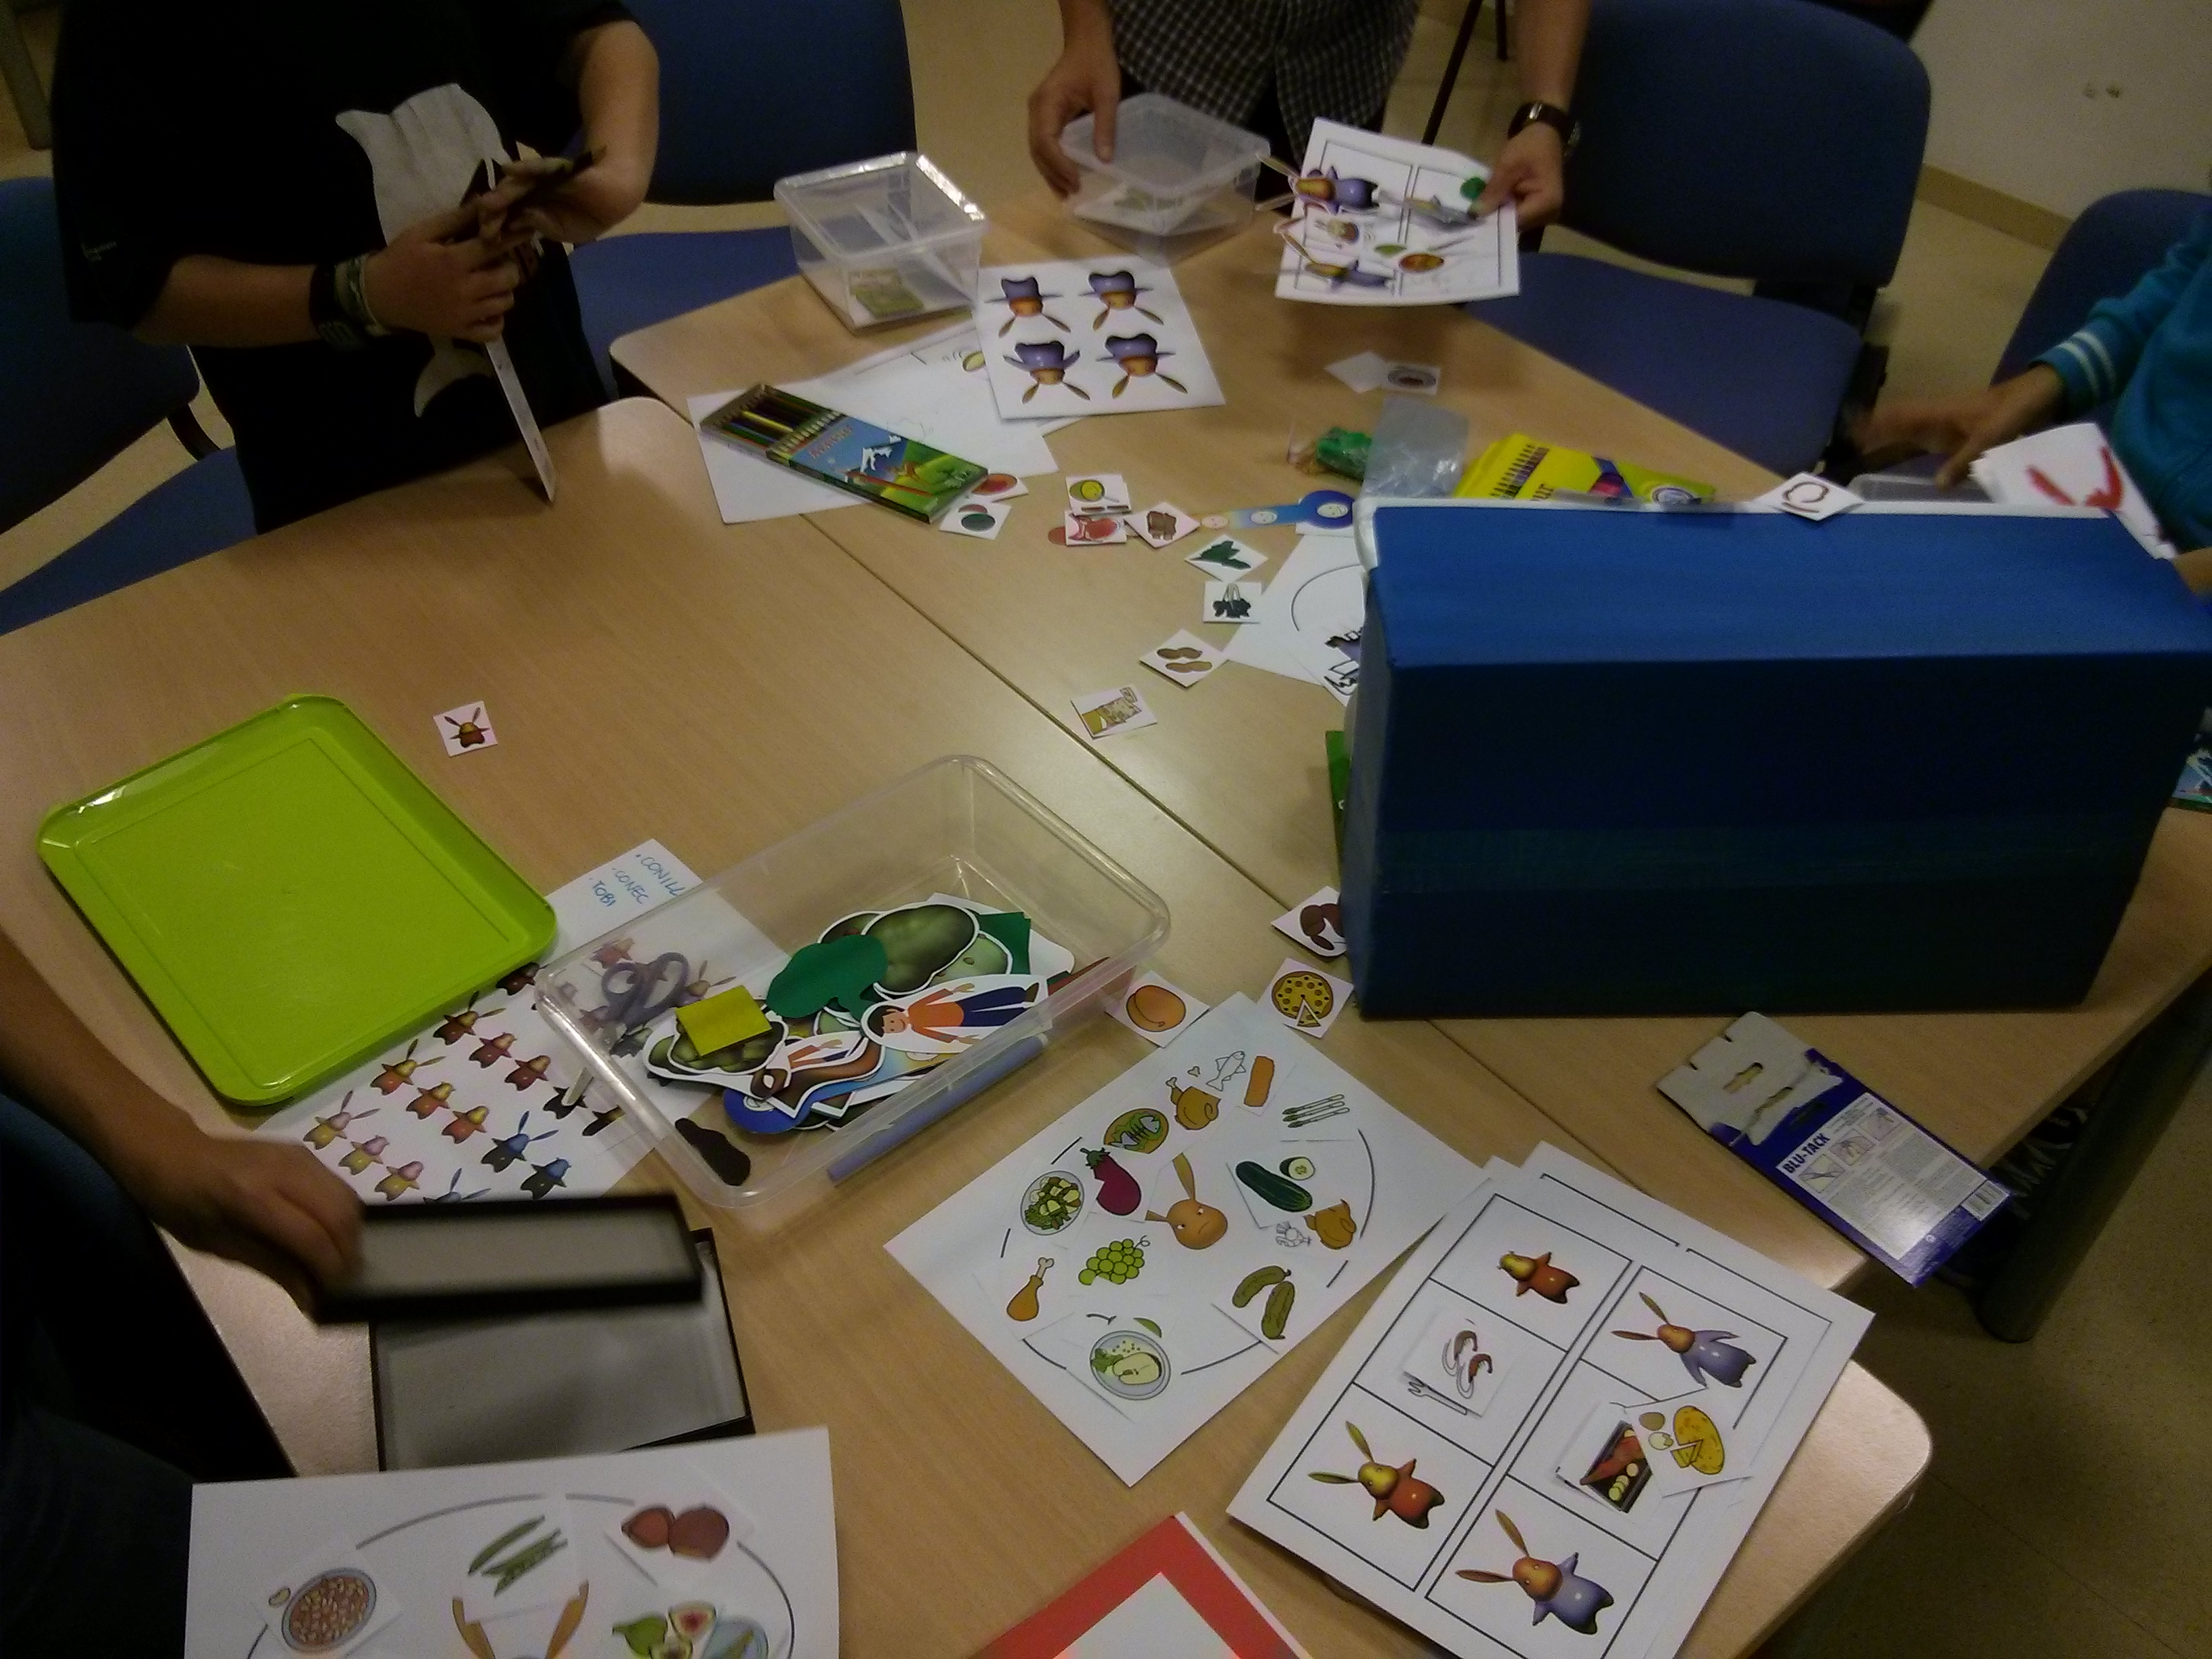
\includegraphics[width=11cm, height=7cm]{immagini/PDchildren.jpg}
\caption{Example of participatory design with children}\label{fig:pdchild}
\end{figure}
Another important aspect is the familiar context in which such co-design activities must be build on. Children must have a reference to which they could ask questions or tell things that otherwise they would not tell strangers (such as a bad opinion on some ideas raised during a discussion), this familiar context could be developed by the presence of a familiar figure as a teacher or a facilitator in the relationship with children.\\
Generally speaking, we can summarize the most important aspects of participatory design with children as follows:
\begin{itemize}
\item \textit{Engagement factors}: the continuous renewing of the session process with the usage of different communication channels that allow the children to maintain a high level focus on the objective and not get bored and that allow the designers to collect as many ideas as possible.
\item \textit{Management factors}: the creation of a familiar environment that allow a more "relaxed" session in which the presence of a familiar figure could interact with children and vice-versa in order to exploit all the opinions (even if bad).
\end{itemize}
As for all participatory design groups of targets, the presence of children allows the designer to build a final product more suitable to the children experience and in line with their point of view. What emerges strongly from studies, is that children are perfectly able to generate design ideas if supported appropriately, even if sometimes these ideas could be difficult to be developed in a real product context, so they need to be revised before an actual implementation.

\subsection{Participatory Design and people with disabilities}
Technology is increasingly being seen as a beneficial addition to the strategies for supporting children with Autism Spectrum Disorders (ASD). Children with ASD typically exhibit an affinity for computers , which provide a safe environment to learn and practice skills that they may find difficult in everyday life. Computers have a number of features particularly appealing for children with ASD, such as the ability to repeat tasks and easily correct errors as pointed out by the National Autistic Society \cite{NAS}. As Malinverni et al. point out from their study with children with special needs, PD activities - if planned properly - can lead to the development of a sense of empowerment and a feeling of competence, both of which reflect a general beneficial effect on the individual, that can derive satisfaction or fun from a useful activity and, at the same time, actually feel the usefulness of his/her contribution \cite{Malinverni}.\\
This approach can often present challenges related with properly defining the role that these children can assume in the design process. Defining the role of children represents a delicate issue since we move in the continuum between overwhelming the child and relegating him in a marginal role, in which his skills are not fully considered. The involvement of ASD children as informants has been reported by several authors \cite{Tredici},\cite{Sedici} and \cite{Venti}, which propose different methods. Methods vary from efforts to get feedback from children about design choices, to the analysis of their preference, the creation of scenarios or the observation of their behavior. The incorporation of these methods permits integrating children's contributions directly into the initial design stages, allowing a deeper influence on the definition of the final product. \\
Approaching PD with people with disabilities comes with a number of challenges that highlight the points to address with more attention whenever performing a series of design sessions in this mindset. The main difficulty is related to the heterogeneity of the participants, with respect to their ages and the degree of their conditions; this factor requires for innovative solutions and, most importantly, for extreme levels of flexibility on the researchers' part - both in terms of planning and of interaction with the
participants. As a consequence, some practical factors must be ensured:
\begin{itemize}
\item The continuity of the team working with the PD group grants a simplification of the entire design setting, by establishing a reassuring personal relation between the members of the whole PD team
\item The gradualness of the design process - and in particular the focus on small, constant changes to the final product - to help giving a sense of completeness and avoiding the dispersion of attention and interest
\item The use of simplified, variated and personalized channels in the process to tackle the difficulty to express the participants' contribution, while helping them understand the structure of the activities they are going to participate in
\item The clarity of the process structure in itself, down to the number of sessions and the individual design activities involved in each session.
\end{itemize}
Benton et al in \cite{Benton} provide designers with a framework that guides them in adapting PD to account for neurodiversity. The framework facilitates the development of PD methods, which direct designers' attention to children's strengths, while supporting their difficulties. Based on the
degree and type of disorders, in fact, strengths and difficulties can be isolated: the PD activity can consequently be shaped around the detailed profile of the participants, in order to leverage on their strong assets and - at the same time - to avoid discouraging them with tasks in which they struggle more.
The most recurring strength in this context is the enhanced creativity of the individuals \cite{Warr}, which hints again at the importance of visual and manual communications skills; their spontaneity and risk-taking tendency may have both beneficial and negative effects, raising the necessity of a controlled
environment in which the potential consequences of these traits are channeled towards positive outcomes. It often occurs that participants show an extreme attention towards details and precision , along with remarkable talent in some very specific area of their interest , and these features can bring much value to the final design \cite{Tredici}. This inclination towards detail is often a signal of what the focus of the PD sessions should be: concentrating on the finer details first and then gradually combining them into a final design is sometimes ideal and preferable to more "top-down-like" approaches.\\
Thus, in general, stress has been put on both the attention to difficulties and the leverage of strengths of subjects suffering from various disabilities, in order to craft the PD activity in the most suitable way possible. It must be noticed that, as all the observed studies point out clearly, not all cases can be summed up in predefined categories and that no ready-to-use solution can exist in dealing with neurodiversity, neither to tackle difficulties nor to exploit strengths. This factor suggests once more how, in the context of PD, it is of vital importance to plan the design process at best, understanding the culture of participants and subsequently tailoring the experience to best fit the whole group, in order to maximize any child's potential for making meaningful contributions to the design process \cite{Benton}. This includes not only considering each individual's strong and weak points, but also possibly a personalization of the means with which each individual interacts and communicates within the PD sessions.
More practical experiences \cite{Malinverni} in the context of PD with people with disabilities have highlighted some aspects that may influence the effectiveness of the process concretely. One of them is the importance of having a regular scheme defined for all the sessions; scheduling meetings close together and using a fixed general structure for all of them often helps creating a sense of continuity for the group, as is also suggested in more general terms by studies mentioning the positive effects of routine elements as introductory recaps and scheduled task checking, for example \cite{Benton}. Temporal proximity of the sessions also helps maintaining the process efficacy, as the participants may find it hard to remember the progresses made over long time periods, depending on the degree of their conditions.\\
A great practical importance has been noticed in the use of physical materials: these kinds of props not only may raise the level of interest of the participants, but also gives a tangible indicator of progression, a sense of achievement and confidence in one's own capabilities. Clearly, the materials must be appropriate for the age and characteristics of the group members; a very intuitive rule-of-thumb is to make materials and prompts essential and clear, as to avoid inducing confusion and, in extreme cases, discouragement in the participants. Depending on the situation and on the composition of the group, it is also possible to vary the type of material used during the design sessions: in particular, it is important to adapt the structure to a more or less restrained way of collecting the participants' inputs, based on their profiles and conditions. The literature over this topic shows some disagreements on the efficacy of using physical schedules explicitly during the design sessions: according to the context, some authors
warn against it as a possible introduction of bias in the participants' behavior within the various sessions \cite{Malinverni}; some other, instead, recommend the use of it as a visual indicator of progress \cite{Benton2} or to create familiarity and establishing a beneficial routine element \cite{Benton}.\\
Whatever choice is made on this point, all studies highlight the vital importance of a continuous and direct communication between the design process coordinators and the participants about the planned activities: this can have the beneficial effects of a schedule, while not introducing any risk of biasing the participants' behavior toward one particular activity or another.
During practical PD sessions, the fundamental role of previous knowledge of the participants is evident: this influences the familiarity with which they approach the design problem the group is called to face together with the designers. Studies have proven that previous knowledge on both the subject of the design process and the logic behind the designed elements - especially if such elements are interactive mechanics of a game or application - may have a direct impact on the improvement of the participants' contributions to the final design \cite{Malinverni}. To this end, it is quite important to consider the possible need to include familiarization sessions in the design process: in general, this is especially required when the object of the design process is technology, as the participants may not be accustomed to the type of devices they will use during the design sessions. Lack of familiarity may, as a direct consequence, induce either over-stimulation due to the novelty of the situation or fear and general uneasiness; needless to say, both conditions are to be avoided, as they are usually harmful to both the process, the individual and the group - especially considering their potential social impact. Effectively, the involvement of children and adults with NDD or various disabilities within a PD framework may generate a mutual advantage for the designers and the design group: at a practical level, the final design benefits from the intervention of a group of people that best reflects the real needs and perspective of the intended user category, as part of the same "culture"; contextually, the participating group undergoes a virtuous process, as their role in a socially-useful task is made more evident, and a sense of individual empowerment and group responsibility is generated in the subjects \cite{Malinverni}. The actual validity of the final design process output may vary a lot, due to the extreme variety of potential end-user conditions. Generally speaking, the similarity of the participants' mindset to the end-user category certainly has the positive aspect of channel the process towards an overall right direction: as Benton et al. observe in their study while validating the PD process, both the actual participants and a consistently comparable group showed very similar behavioral responses upon interacting with the final design product. Still, though, those who did not participate in the design pointed out a considerably higher number of desired features - either missing or different from expectation/desire - with respect to the group which had an active part in the design process \cite{Benton2}. This experience suggests extreme caution while measuring the positive effect of PD methods on the design pipeline and especially on the end product quality, as the improvement might not be as evident as expected, and - according to the very context of execution of the design process - may even end up being negligible or irrelevant.\\

As we explored the general features assumed by the PD techniques involving people with
disabilities, it becomes really clear that most models proposed in literature have been
crafted with children or adolescents with special needs in mind. However, it must be noticed that - as several studies point out, e.g.\cite{Diciasette},\cite{Diciotto} and \cite{Diciannove} - most
of the general indications we listed above work quite well for both children, young adults
and even seniors suffering from NDD or disabilities in general. Of course, this factor is
rendered quite uncertain by the heterogeneity of the community these kind of design
processes are involving; still, some common features emerge and allow us to consider the
possible guidelines provided by a number of research studies as suitable for people with
disabilities of virtually any age. In particular, recurring common elements in studies with
adult subjects with disabilities include:
\begin{itemize}
\item the need for multiple communication channels to avoid limitations deriving from
the difficulties of expressing concepts, and in particular the necessity of adapting
traditional methods to a suitable level, based on the specific group
\item the importance of practical design sessions alongside more general interviewbased
ones
\item the beneficial effect of using props and technological probes towards an improved
contribution to the design by participants in direct and indirect ways
\item the importance of structure clarity within and across sessions
\item the positive effects on both the design and the group, in the latter case particularly
the induction of empowerment and feeling of competence
\end{itemize}
Having established a general equivalence - set apart the due considerations about the
appropriateness of the activities level with respect to the individuals in the group -, we
can observe how several researchers have provided useful frameworks and guidelines to
follow whenever undertaking a new PD study. Benton et al. \cite{Benton2} outline some "best practices" to remember for PD sessions by extracting
them from multiple experiences with groups of subjects showing varying degrees of
developmental disorders:
\begin{itemize}
\item Value is attributed to the process by ensuring that participants understand and
are interested in what they are doing, meaning that it is vital to ensure that they
are familiar with the subject and are stimulated by it to constructively participate
to every session.
\item Concrete thinking must be preferred to abstract thinking as it is closer to the way
most people with disabilities interact with the social environment; also, it allows
for very direct feedback, which - despite being potentially discouraging for
somebody - may be much more useful in design processes as it favors quick and
to-the-point information collection.
\item Structure organization using visual means is useful to create continuity and
involvement in the group; however, this has proven not to be the case in some
practical experiences \cite{Malinverni} and may strongly depend on the nature of the group
and the context in which the process takes place.
\item It is also very advantageous to the process to involve enthusiastic and very flexible
people from the teaching/tutoring context, as this could help leverage the activities
on the strong suits of the individual participants, thus building up their confidence
and willingness to contribute.
\end{itemize}
Focusing on the
variety of interests of the participants - especially when dealing with younger subjects -
can help channel their willingness to participate in design activities instead of inducing a
feeling of uneasiness by "forcing" them to take part in an activity that may be perceived
as unpleasant, unfamiliar or even scary. The framework builds over this key factor to obtain a well-defined infrastructure of the
design activity: the next factor to consider is the integration of the participants' social
background as a whole: families, tutors and educators are included in the process directly,
in order to take full advantage of the existing relationships between them and the
participants. This way, the social aspect is leveraged to produce new constructive types of
contributions; at the same time, the additional human factor can make certain social
situations and contexts very evident, thus allowing to tailor the design activities according
to the constraints and opportunities induced by the social backgrounds of every subject
involved.
Having laid out a structure specifically shaped around the personal and social spheres of
the participants, the focus can be moved to the result of the process, and in particular to
the efficacy, flexibility and suitability of the resulting product. These factors are the core
of the product design analysis: with the inclusion of the extended social background of
the participants, these measures of adequacy and suitability to the given needs can be
explored more in depth; in fact, the design activities are planned since the beginning to
evolve in an emulated social environment , that allows to better understand the real-life
effects of the designed product or service.
After that, the framework invites to bring the design to the real social and physical
environments , so that the details neglected by the previous "approximations" are
observed and accounted for. This includes the analysis of interactions and engagement with the artifact or service in an everyday context, from which we can derive information
on actual usability and usefulness.
The key idea of focusing the design work on the involved subjects' strengths as opposed
to their difficulties is also central in Benton et al. \cite{Benton}, whose research outlines a flexible
framework, adaptable according to the individual participants' profiles in order to
simultaneously exploit the multiple strong characteristics exposed by neurodiversity and
reduce the attrition posed by obvious difficulties.
The overall framework proposed by the study focuses on the key concepts of
understanding neurodiverse cultures as different structures for thinking and behaving,
with associated strong assets and weaknesses; and tailoring the activities to the
individuals , as to account for their unique and distinctive characteristics. This allows to
draw a very detailed picture of the group, having explored the needs, interests and skills
of its members thoroughly and at multiple levels: both "generally" as part of a culture
presenting very peculiar common features and "specifically" as an individual equipped
with his/her personal set of skills and vulnerabilities.
This type of framework provides a highly flexible way of proceeding when structuring a
PD activity, to the point that the activities can be adapted and shaped around the
individual profiles of the participants.
Breaking out the details of the involved subjects' cultures is relevant to highlight very
practical elements, essential to the subjects themselves, to be accounted for in many
situations; at the same time, the involvement of additional support from adults, parents,
tutors or educators and the customization of activities allow to take full advantage of the
whole skillset of the individual, as well as the typical characteristics associated with his/her
background culture. All the features extracted with this method necessarily reflect both the complexity of the
culture the individual belongs to and his/her specific individuality.
The framework effectively describes a way to generate PD methods rather than defining
a unique and generalized model to adapt to; this reflects the general mindset of PD quite
well, as it is a way to give value to each participant based on his/her actual skills and ability
to better reflect needs that are typical of the culture he/she belongs to. Despite having a tendency to produce "disposable" process structures, the researchers'
experience with the framework points out how its employment and gradual enrichment
contributes - as a sort of by-product - to enlarging the base knowledge of designers
engaging with neurodiversity, by extracting and modeling the general traits of the
expertise in this field longitudinally.
Among the outlined models for PD, the recurring element is the focus on the extreme
importance that the need extraction process assumes when structuring design process
involving people with disabilities.
As most perspectives focus on the strengths and difficulties of the participants in order to
craft the design activities and tasks accordingly, it appears very clearly that the key to good
PD is accounting in a very focused way for the special necessities exhibited by them and
tailoring the experience as best suits each single one of them.
Variety is indeed the key to success, as it perfectly reflects the landscape of disability with
its exceptional range of perspectives and unique conditions; no real general method is
possible in such context, as generalization would necessarily impose limits to the possible
extent of an individual's contribution, as it would in fact be an enforcement of a mindset
and a behavior that would prove unnatural or simply incomprehensible to him/her.

 